

\section{Etapa 1}

\begin{figure}[H]
\centering
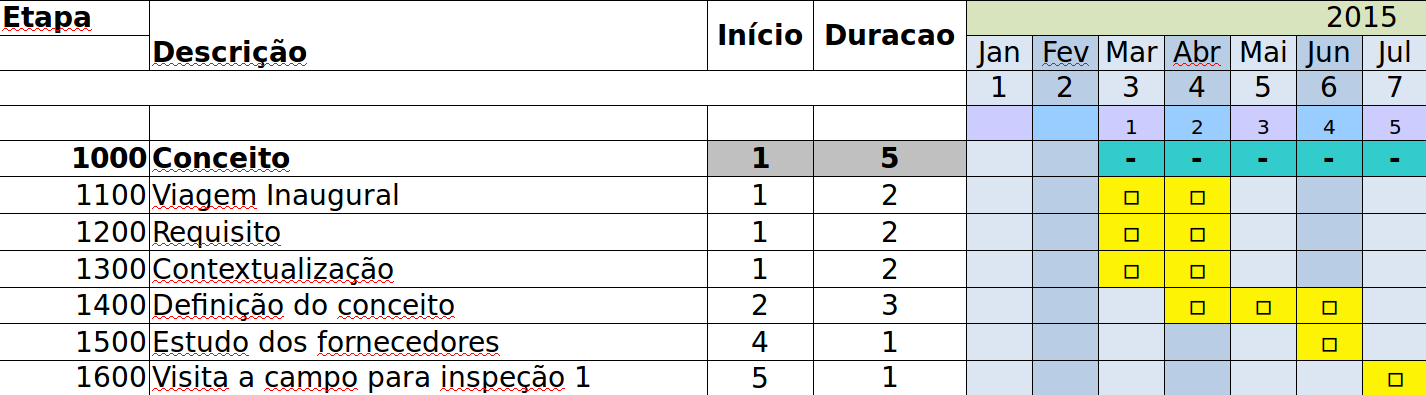
\includegraphics[width=0.9\columnwidth]{figs/etapa1}
\end{figure} 

\textbf{1000 Conceito:} A etapa 1000 do projeto foi executada como prevista. O
objetivo da etapa foi a determinação dos requisitos do problema e concepção de
possíveis soluções. As seguintes trabalhos foram executados dentro desta etapa

\textbf{1100 Viagem Inaugural:} Assinatura do termo inaugural do projeto e
análise em campo da problemática

Etapa executada como previsto. 

\begin{figure}[H]
\centering
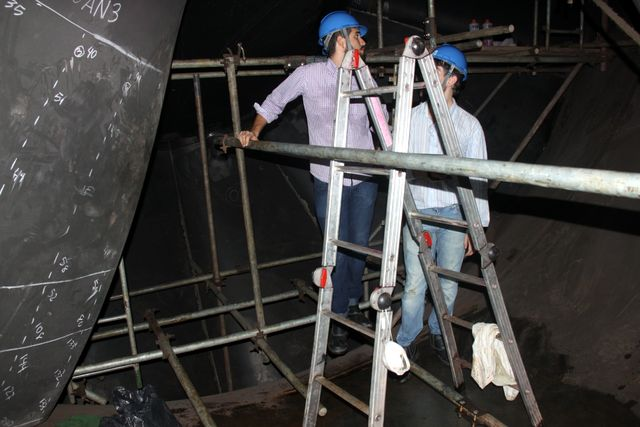
\includegraphics[width=0.6\columnwidth]{figs/img_4967}
\caption{Pesquisadores analisando o ambiente.}
\end{figure}


\textbf{1200 Requisito:} Fazer levantamento dos requisitos que afetam a
instalação e utilização de um robô dentro circuito hidráulico.

Etapa executada como previsto. Foram levantados todos os requisitos de acesso,
ambiente e processo de coating.

\textbf{1300 Contextualização:} Levantamento das tecnologias existentes no para
aplicações de revestimento em ambientes confinados.

Etapa executada como previsto. Diversas tecnologias foram pesquisadas, como o
robô scompi da hidroquebec. Nenhuma das soluções atuais atendiam os requisitos
de operação do projeto.

\textbf{1400 Definição dos conceitos:} Definição de uma solução de um robô capaz
de operar no ambiente e realizar tarefas de revestimento.

Etapa executada como previsto. Foram levantados 3 conceitos viáveis, os quais
foram analisados chegando ao conceito proposto dentro do projeto. Utilizar um
manipulador industrial, acessando o circuito hidráulico pela escotilha de
acesso, com movimentação através de trilhos modulares e alinhamento, mapeamento
e planejamento de trajetória baseado em scan 3D a laser do ambiente.

\begin{figure}
\centering
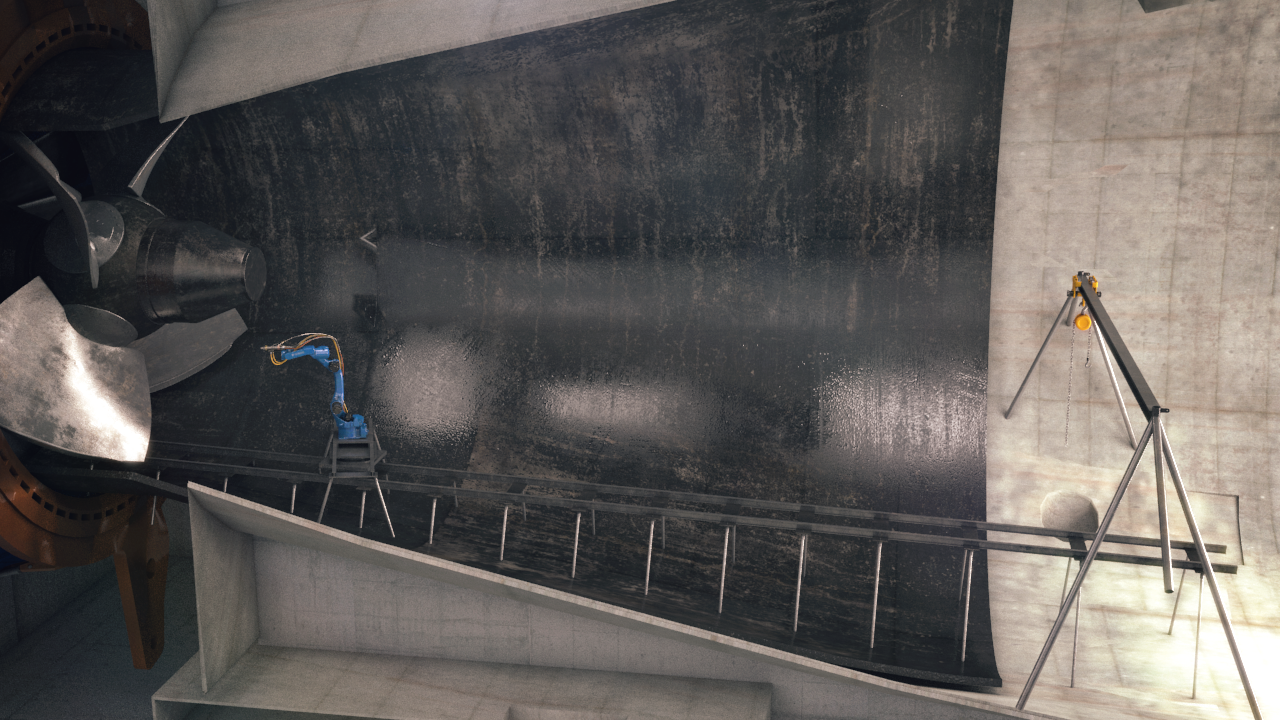
\includegraphics[width=0.9\columnwidth]{figs/turbine_evo}
\caption{Solução conceito.}
\end{figure}

\textbf{1500 Estudo dos fornecedores:} Definição dos fornecedores do equipamento
necessário para a pesquisa

Etapa executada como previsto. Foram analisados mais de 50 modelos de
manipuladores distintos, sendo que 5 atendiam os requisitos do problema como
possíveis soluções.

\begin{figure}[h!]
\centering
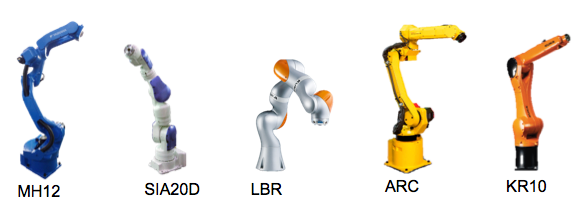
\includegraphics[width=0.9\columnwidth]{figs/robots}
\caption{Possíveis modelos de manipuladores que atendem os requisitos.}
\end{figure}

\section{Etapa 02}

\begin{figure}[H]
\centering
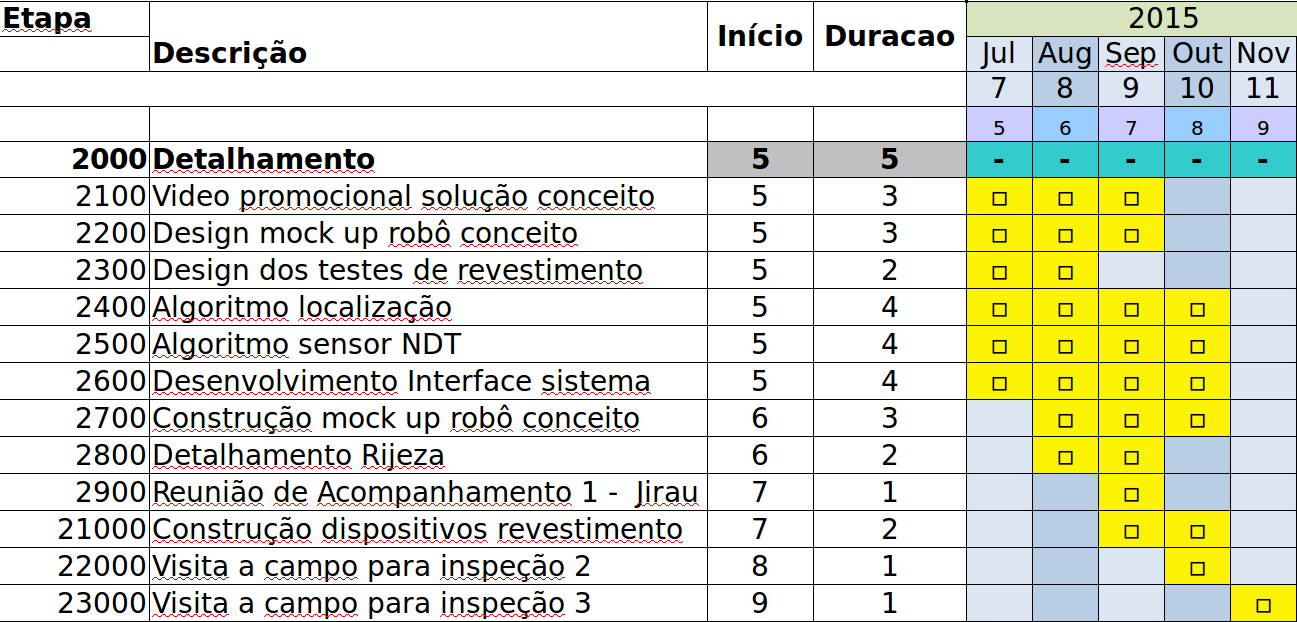
\includegraphics[width=0.9\columnwidth]{figs/etapa2}
\end{figure} 

\textbf{2000 Detalhamento:} A etapa 2000 do projeto foi executada existindo
variações entre previsto e executado. O objetivo da etapa foi a análise das
proposições mediante estudos teóricos e design detalhado da possível solução e sistema

\textbf{2100 Video promocional solução conceito:} Animação 3D da solução
conceito

Houve atraso no processo de contratação e aprovação do script. A tarefa foi
executada com 3 meses de atraso. Entretanto, o mesmo não impactou no projeto,
pois não era uma tarefa de pré-requisito.

\textbf{2200 Design mock up robô conceito:} Design em CAD / Solidworks do
conceito do robô

Tarefa executada como prevista. Foram realizado diversos designs para possíveis
bases para a solução conceito, assim como análises geométricas, cinemática,
dinâmica e de manipulabilidade para definir o manipulador.

\begin{figure}\centering
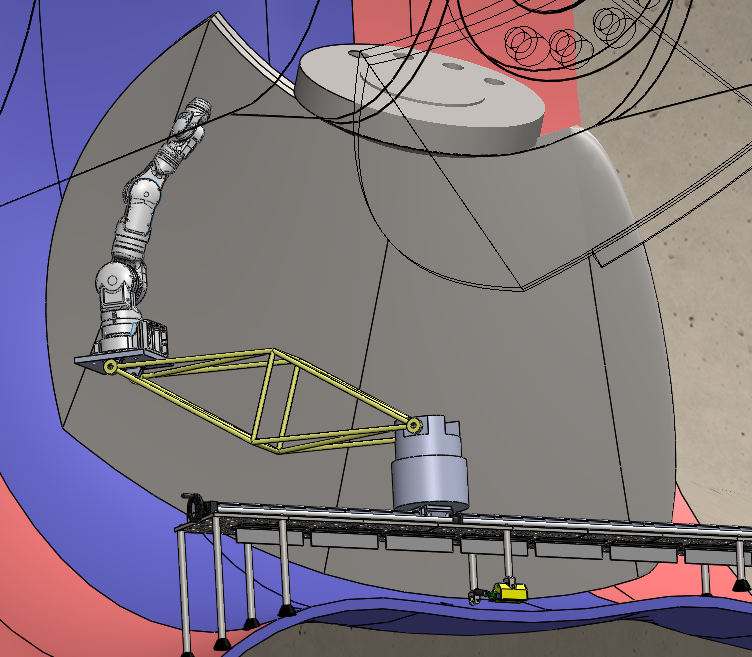
\includegraphics[width=0.6\columnwidth]{figs/EMMA_Base_Conceito_PRR}
\caption{Possível base para o manipulador dentro do ambiente do circuito
hidráulico.}
\end{figure} 


\textbf{2300 Design dos testes de revestimento:} %TODO DARLAN

\textbf{2400 Algoritmo de localização:} definir o algoritmo/técnica que irá
localizar o robô com relação a turbina.

Tarefa executada como prevista. Foi determinado que o melhor e mais preciso
método é escanear o robô e a pá com um laser de metrologia e a estimar posição
relativa das nuvens de pontos resultantes.

\begin{figure}[H]
\centering
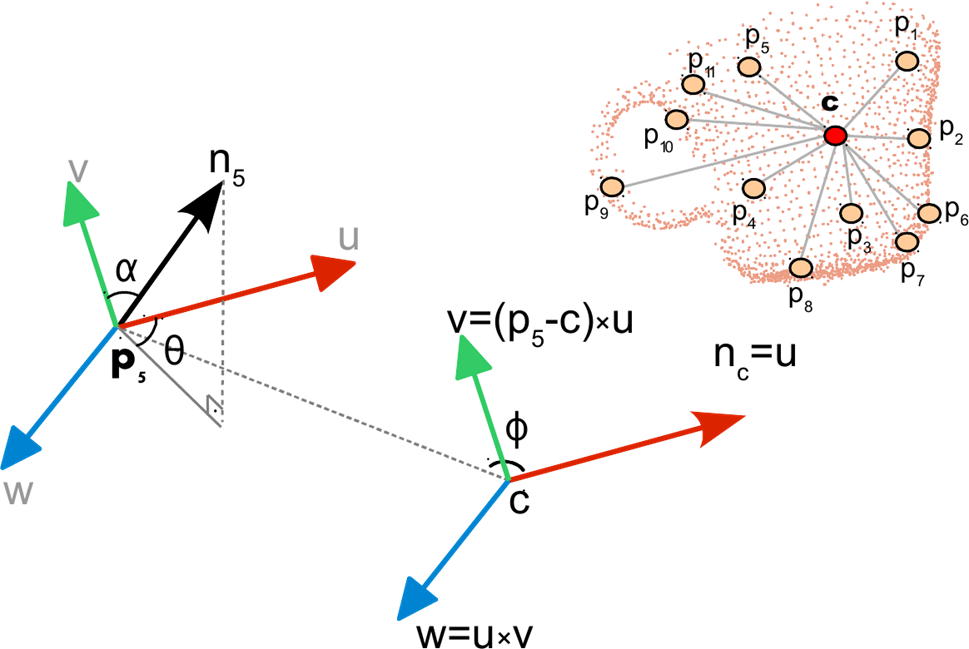
\includegraphics[width=0.6\columnwidth]{figs/pc_position}
\caption{Posição relativa entre duas nuvens de pontos.}
\end{figure} 

\textbf{2500 Algoritmo sensor NDT:} Algoritmo que irá avaliar e mapear a
qualidade do revestimento.

Tarefa executada como prevista. Foi determinado que o método mais eficiente é
utilizar um humano para rapidamente realizar uma amostragem de alguns pontos com
sensor ultra-som manual. A solução robótica seria em uma alusão “matar um mosquito com basuca”.

\textbf{2600 Desenvolvimento Interface sistema:} Interface gráfica de controle e
utilização do sistema

Essa tarefa foi estendida para 8 meses, se tornando uma teses de mestrado dada
sua complexidade. A solução conceito possui um volume muito grande de interação
e informação para o usuário. Logo, adotou-se um estudo metódico,
estabelecendo-se toda a metodologia para determinar a interface e como cada
informação será representada.

\textbf{2700 Construção mock up robô conceito:} Construção do mock up do robô
que aplica o revestimento

Tarefa executada como previsto. Foi construído todo o ambiente do circuito
hidráulico e manipulador através de impressão 3D em uma escala 1:20.

\begin{figure}[h!]
\centering
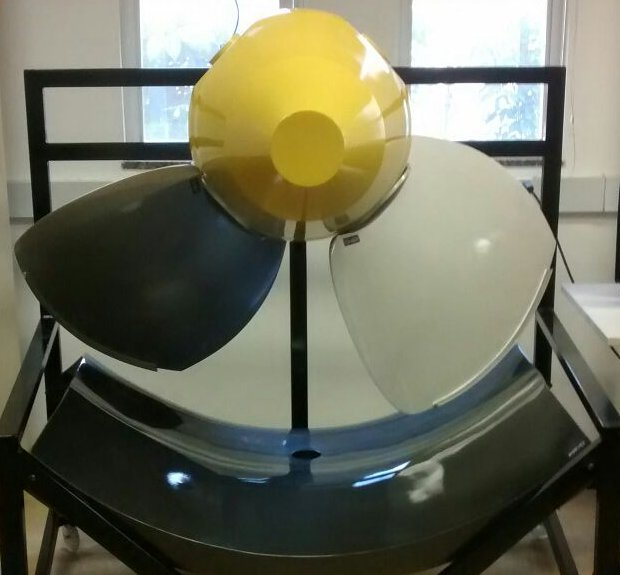
\includegraphics[width=0.6\columnwidth]{figs/maquete}
\caption{Maquete utilizada no desenvolvimento do conceito.}
\end{figure} 

  

\textbf{2800 Construção dos dispositivos de revestimento:} %TODO DARLAN

\textbf{2900 Reunião de acompanhamento:} Reunião de acompanhemento to projeto

Tarefa executada como prevista. 

\begin{figure}\centering
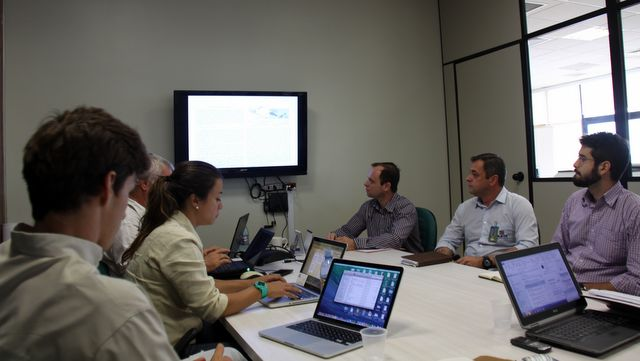
\includegraphics[width=0.6\columnwidth]{figs/img_4836}
\caption{Reunião de acompanhamento em Jirau.}
\end{figure} 

\section{Etapa 03} 

\begin{figure}[H]
\centering
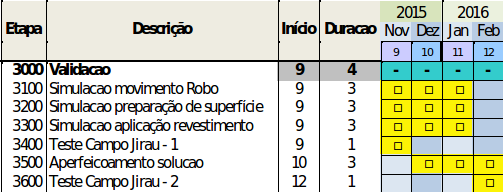
\includegraphics[width=0.9\columnwidth]{figs/etapa3}
\end{figure} 

\textbf{3000 Detalhamento:} A etapa 3000 do projeto foi executada existindo
variações entre previsto e executado. O objetivo da etapa é validação da solução
detalhada através de simulação e experimentos.

\textbf{3100 Simulação movimento robô:} 
Simulação dos movimentos do robô sobre a turbina, verificando limites e singularidades

Tarefa executada como prevista. Foi utilizado o simulador Openrave.  

\textbf{3200 Simulação preparação de superfície:}

DARLAN 

\textbf{3300 Simulação aplicação revestimento:}

DARLAN 

\textbf{3400 Teste de Campo Jirau 01:} Teste da solução  em Jirau sobre
condições reais de operação

Tarefa executada antes do previsto. Os testes de campo foram executados durante
a viagem de acompanhamento que ocorreu na etapa 2900. Foram testados os
conceitos de acoplamento magnético e mapeamento 3D com laser scanner.

\begin{figure}
\centering
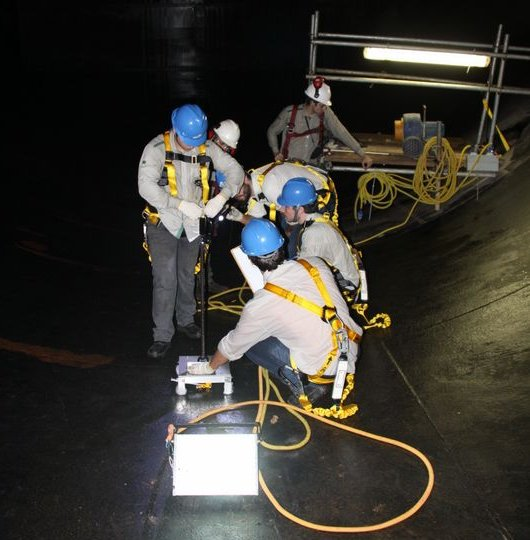
\includegraphics[width=0.6\columnwidth]{figs/base}
\caption{Teste de campo com a base  magnética}
\end{figure}

\textbf{3500 Aperfeiçoamento da solução:}
Aperfeiçoamento da solução baseado nos resultados dos testes de campo 

Tarefa atrasada em 1 mês com impacto de atraso de 1 mês no projeto. O cálculo da
posição relativa entre o robô e a pá, baseado em dados reais do sensor de
metrologia testado em campo, está com um erro de 0,1-0,2 graus o que resulta em
um erro de posição da extremidade do manipulador na ordem de centímetros. A
ordem de grandeza desejada para poder fazer reparo do perfil hidráulico é em
milímetros. Logo, as técnicas de alinhamento continuando sendo aprimoradas.

\begin{figure}\centering
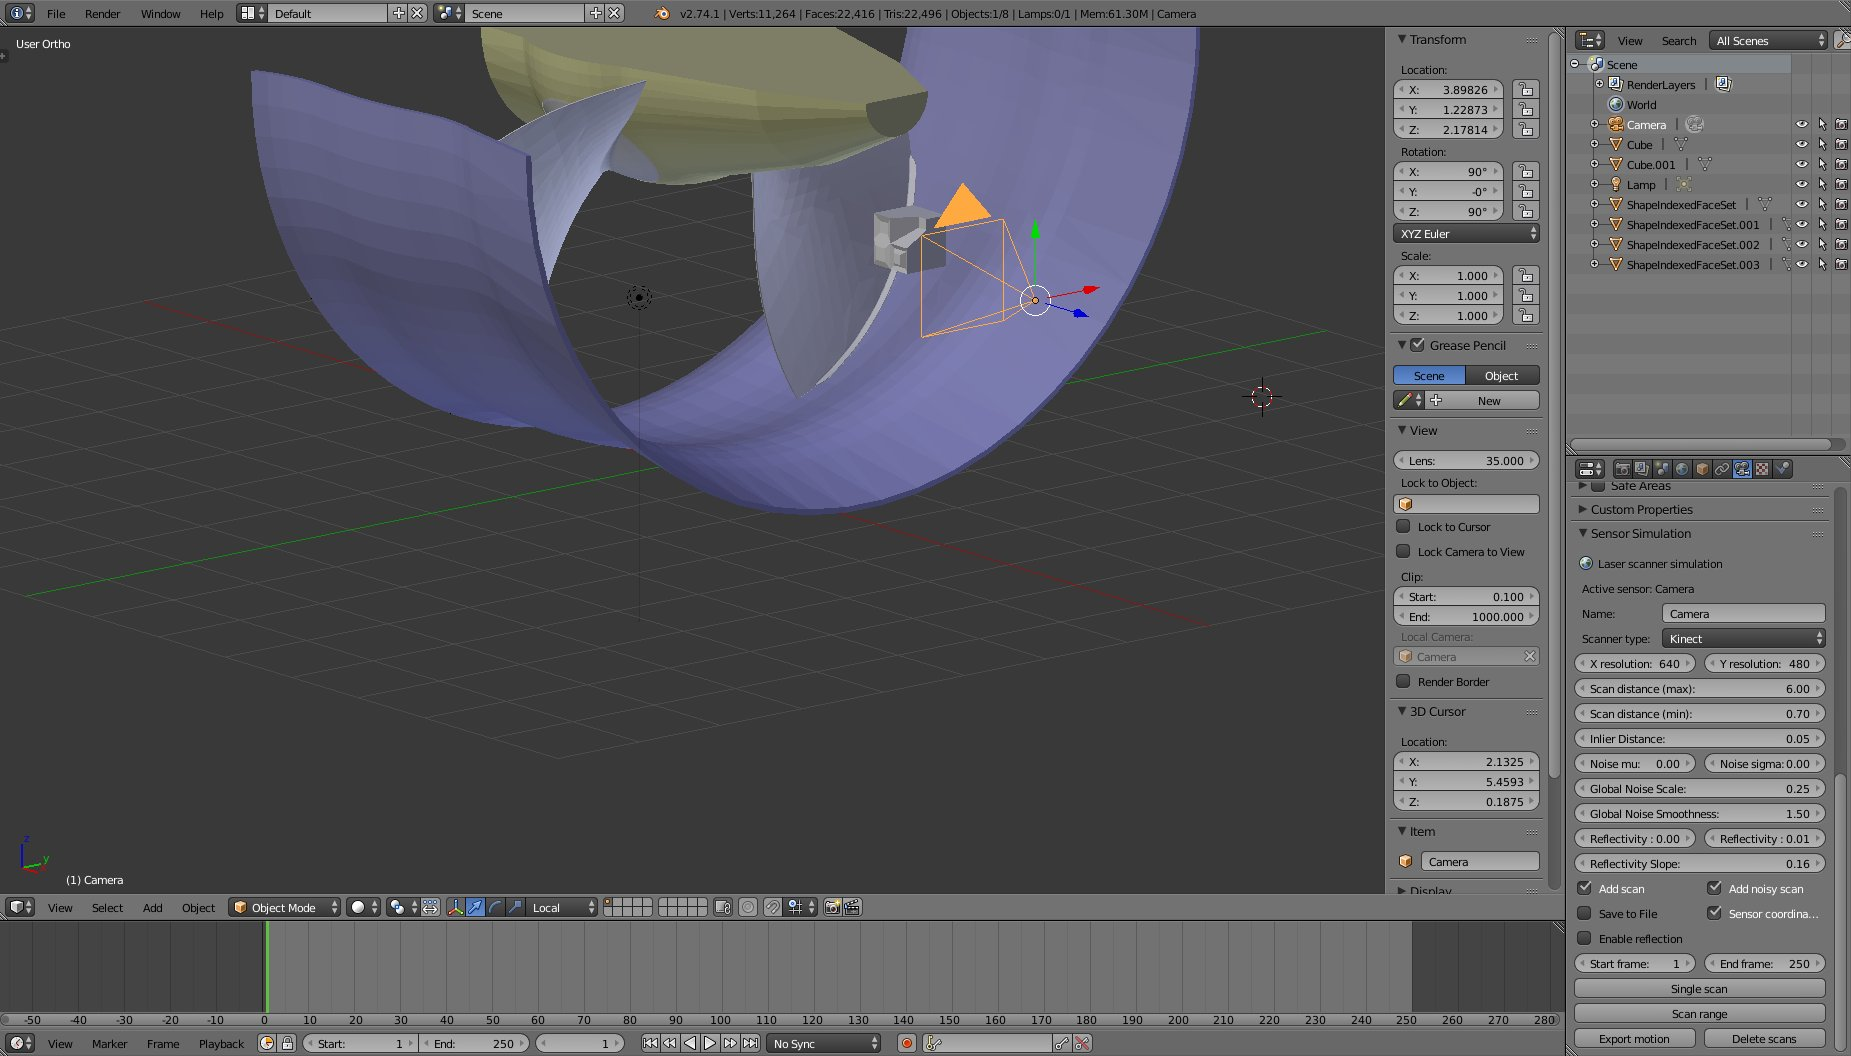
\includegraphics[width=0.6\columnwidth]{figs/blensor_screen}
\caption{Estimando posição relativa usando um simulador para análise dos
resultados.}
\end{figure} 


\textbf{3600 Teste de Campo Jirau 02:} Teste da solução  em Jirau sobre
condições reais de operação.

Tarefa cancelada. As informações necessárias para esta fase do
projeto foram coletadas durante a o teste de campo 01. 

\section{Etapa 04} 

\begin{figure}[H]
\centering
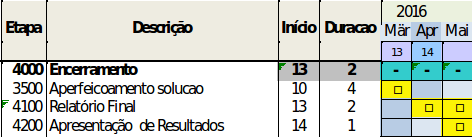
\includegraphics[width=0.7\columnwidth]{figs/etapa4}
\end{figure} 

\textbf{4000 Encerramento:} A etapa 4000 do projeto foi executada existindo
variações entre previsto e executado. Inicialmente esta etapa era para ser
iniciada em março e encerrada em abril. Entretanto a mesma sofreu um atraso de 1
mês devido a necessidade de mais tempo para encerrar a etapa de aperfeiçoamento
da solução. O objetivo da etapa é preparar os relatórios finais e artigos acadêmicos do projeto.

\textbf{4100 Relatório Final:} Relatório de encerramento do projeto no formato
P\&D Aneel e artigos acadêmicos.

Etapa executada como prevista. 

\textbf{4200 Apresentação dos resultados:} Difusão dos conhecimentos.

Etapa executada como prevista. Foi realizado um evento na faculdade de Porto
Velho, onde os pesquisadores do projeto EMMA realizaram uma aula de pesquisa
aplicada explicando as pesquisas desenvolvidas, seus conceitos e resultados.
 